\documentclass[12pt, a4paper]{article}

\usepackage[margin=1in]{geometry}
\usepackage{hyperref}
\usepackage{titlesec}
\usepackage{enumitem}
\usepackage{booktabs}
\usepackage{xcolor}
\usepackage{microtype}
\usepackage{amsmath}
\usepackage{amssymb}
\usepackage{fancyhdr}
\usepackage{array}
\usepackage{longtable}
\usepackage{listings}
\usepackage{tikz}
\usetikzlibrary{positioning, arrows.meta}

\hypersetup{
    colorlinks=true,
    linkcolor=blue!70!black,
    urlcolor=blue!70!black,
}

\pagestyle{fancy}
\fancyhf{}
\fancyhead[R]{sujeet.banerjee@gmail.com
\\
sujeet.banerjee.professional@gmail.com}
\fancyhead[L]{Agentic AI Bootcamp}
\fancyfoot[R]{\thepage}
\fancyfoot[L]{RAG: Reranking \& Retrieval Evaluation}
\renewcommand{\headrulewidth}{0.4pt}
\renewcommand{\footrulewidth}{0.4pt}

\title{\textbf{RAG Reranking and Retrieval Evaluation}\\
\large From Top-$K$ Retrieval to Context Precision and Context Recall}
\author{Detailed Notes - Agentic AI Bootcamp}
\date{}

\lstset{
    basicstyle=\ttfamily\small,
    columns=fullflexible,
    keepspaces=true,
    frame=single,
    breaklines=true,
    showstringspaces=false
}

\begin{document}

\maketitle
\tableofcontents
\newpage

\section{Why Reranking Exists}

A Retrieval-Augmented Generation (RAG) system normally has three broad stages:

\begin{enumerate}
    \item \textbf{Retrieve candidates} from a large document collection.
    \item \textbf{Rerank the candidates} according to their relevance to the user's query.
    \item \textbf{Generate an answer} using the best retrieved context.
\end{enumerate}

A useful mental model is:

\begin{center}
\textbf{Retriever = candidate generator}\\
\textbf{Reranker = relevance judge}\\
\textbf{Generator = answer synthesizer}
\end{center}

The key reason for separating these stages is that retrieval and ranking optimize different objectives.

\begin{itemize}
    \item The first-stage retriever should emphasize \textbf{recall}: do not miss potentially useful information.
    \item The reranker should emphasize \textbf{precision}: among the candidates, put the most useful information first.
    \item The generator should use the final context to produce a grounded answer.
\end{itemize}

\section{The Two-Stage Retrieval Architecture}

A typical RAG pipeline can look like this:
\\
\begin{center}
    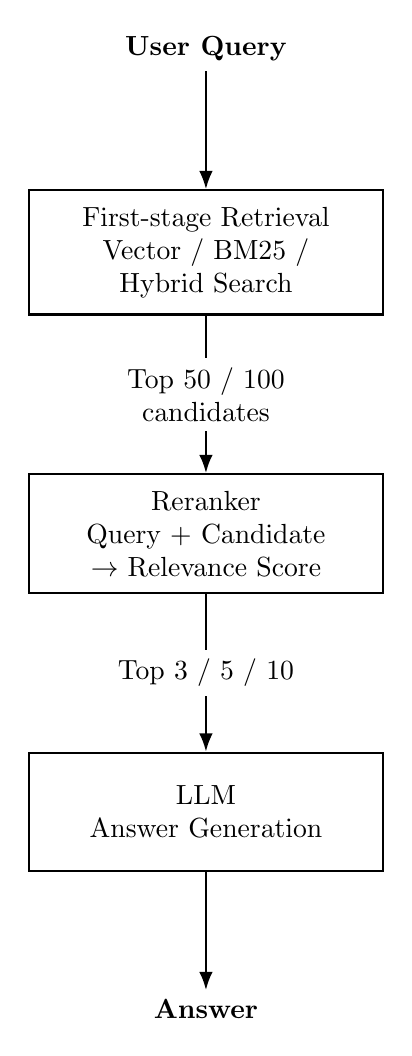
\begin{tikzpicture}[
        % Define common styles for the nodes and text
        node distance=1.5cm,
        box/.style={draw, rectangle, thick, align=center, minimum width=4.5cm, minimum height=1.5cm, inner sep=6pt},
        textnode/.style={align=center, font=\bfseries},
        arrow/.style={-Latex, thick}
    ]
    
        % Define the nodes
        \node[textnode] (query) {User Query};
        
        \node[box, below=of query] (retrieval) {First-stage Retrieval \\ Vector / BM25 / \\ Hybrid Search};
        
        \node[box, below=2cm of retrieval] (reranker) {Reranker \\ Query + Candidate \\ $\rightarrow$ Relevance Score};
        
        \node[box, below=2cm of reranker] (llm) {LLM \\ Answer Generation};
        
        \node[textnode, below=of llm] (answer) {Answer};
    
        % Draw the arrows with labels
        \draw[arrow] (query) -- (retrieval);
        
        \draw[arrow] (retrieval) -- node[fill=white, align=center] {Top 50 / 100 \\ candidates} (reranker);
        
        \draw[arrow] (reranker) -- node[fill=white, align=center] {Top 3 / 5 / 10} (llm);
        
        \draw[arrow] (llm) -- (answer);
    
    \end{tikzpicture}
 \end{center}

% \begin{verbatim}
%                          User Query
%                              |
%                              v
%                  +----------------------+
%                  | First-stage Retrieval|
%                  | Vector / BM25 /      |
%                  | Hybrid Search        |
%                  +----------------------+
%                              |
%                        Top 50 / 100
%                        candidates
%                              |
%                              v
%                  +----------------------+
%                  |      Reranker        |
%                  | Query + Candidate    |
%                  | -> Relevance Score   |
%                  +----------------------+
%                              |
%                       Top 3 / 5 / 10
%                              |
%                              v
%                  +----------------------+
%                  |       LLM            |
%                  | Answer Generation    |
%                  +----------------------+
%                              |
%                              v
%                           Answer
% \end{verbatim}

For example, a collection may contain 10,000 chunks. A vector database might retrieve the best 50 candidates. A reranker can then examine those 50 candidates more carefully and select the best 5 for the final LLM prompt.

This is generally preferable to asking the vector database to directly return only five chunks, because the first stage can deliberately optimize for \textbf{recall} while the second stage restores \textbf{precision}.

\section{Why Vector Similarity Alone Is Not Enough}

Embedding retrieval answers a question approximately like:

\begin{quote}
``Which documents are semantically similar to this query?''
\end{quote}

That is useful, but semantic similarity is not identical to answer relevance.

Consider the query:

\begin{quote}
\textit{What is the company's policy for employees working remotely from another country?}
\end{quote}

A first-stage retriever might return:

\begin{enumerate}
    \item Working From Abroad
    \item Remote Work Policy
    \item Employee Travel Policy
    \item Office Attendance Policy
    \item International Payroll
\end{enumerate}

All five can be semantically related to the query. However, only some may contain the precise information required to answer it.

A reranker can compare the query directly against each candidate and assign a relevance score:

\begin{center}
\begin{tabular}{p{0.62\textwidth}c}
\toprule
Candidate & Example relevance score\\
\midrule
Working From Abroad & 0.91\\
Remote Work Policy & 0.84\\
Employee Travel Policy & 0.54\\
International Payroll & 0.37\\
Office Attendance Policy & 0.29\\
\bottomrule
\end{tabular}
\end{center}

The exact numerical scores are illustrative. The important idea is that the reranker produces a \textbf{query-dependent ordering}.

\section{What Does Cohere Use for Reranking?}

Cohere provides dedicated \textbf{Rerank models}. These are neural relevance models designed specifically for ranking documents with respect to a query.

The current Cohere documentation lists, among others:

\begin{itemize}
    \item \texttt{rerank-v4.0-pro}
    \item \texttt{rerank-v4.0-fast}
    \item \texttt{rerank-v3.5}
\end{itemize}

Cohere describes Rerank as a semantic ranking model: given a query and a list of documents, it predicts relevance and returns the documents ordered from most to least relevant.

The important architectural point is:

\begin{quote}
\textbf{Cohere Rerank is model-based, but it is not same as a general-purpose LLM (i.e. it does not ``haev generative capabilities'').}
\end{quote}

It is better described as a \textbf{specialized transformer-based relevance/reranking model}, which is a trained Neural-Network.

\subsection{Query and Document Are Considered Together}

The key distinction from embedding retrieval is that the reranker directly considers the query and candidate document together.

Conceptually:

\[
(\text{Query},\text{Document}) \longrightarrow \text{Relevance Score}
\]

Cohere describes this as applying \textbf{cross-attention} for fine-grained ranking.

By contrast, a typical embedding retrieval flow is:

\[
\text{Query} \longrightarrow \mathbf{q}
\]

\[
\text{Document} \longrightarrow \mathbf{d}
\]

followed by a similarity calculation such as:

\[
\operatorname{sim}(\mathbf{q},\mathbf{d})
\]

The reranker therefore performs a more direct query-document interaction.

\section{Is Cohere Rerank an LLM?}

Well, not precisely! LLM is a \textbf{Large Language Model}, while Reranker is usually a Transformer based model, which is a trained \textbf{Neural Network} to predict scores based on the relevancy of the chunks with respect to the user \textit{query}. 

Thus,

\begin{center}
\textbf{Reranker = transformer-based relevance model}\\
\textbf{Generator = general-purpose generative LLM}
\end{center}

\begin{longtable}{p{0.22\textwidth}p{0.68\textwidth}}
\toprule
\textbf{Component} & \textbf{Primary job}\\
\midrule
Embedding model & Converts query/documents into vectors.\\
Vector database / search engine & Retrieves candidate documents efficiently.\\
Reranker & Scores candidate documents for query relevance and reorders them.\\
Generative LLM & Uses the selected context to generate the final response.\\
\bottomrule
\end{longtable}

Yes, there are several popular implementations and models specifically designed or commonly used for LLM-based reranking:

\begin{enumerate}
    \item \textbf{RankGPT:} A widely used methodology that leverages frontier models (like GPT-4) to perform listwise ranking of retrieved passages. Orchestration frameworks like \texttt{LlamaIndex} offer built-in modules (like \texttt{RankGPTReranker} or \texttt{LLMRerank}) that implement this out-of-the-box.

    \item \textbf{RankZephyr:} An open-weight model specifically distilled to replicate the ranking capabilities of larger models. This allows developers to run a highly capable LLM reranker locally without the heavy API costs of a frontier model.

    \item \textbf{Qwen3 Reranker:} A family of models that use a generative LLM architecture to score document relevance based on the probability of generating a "yes" versus "no" for a query-document pair.
    
\end{enumerate}

% Trade-off b/w NN and LLM based rerankers.
\begin{table}[htbp]
\centering
\renewcommand{\arraystretch}{1.5}
\begin{tabular}{@{}p{0.25\linewidth}p{0.35\linewidth}p{0.35\linewidth}@{}}
\toprule
\textbf{Consideration} & \textbf{Traditional Cross-Encoders} & \textbf{LLM Rerankers} \\ 
\midrule
\textbf{Latency} & Usually adds tens to low-hundreds of milliseconds per query. & Can take seconds, depending on the model size and candidate pool. \\
\textbf{Cost} & Very cheap to run, easily hosted on moderate hardware. & Can become prohibitively expensive due to high token usage per query. \\
\textbf{Out-of-Domain Accuracy} & Can struggle if the domain vocabulary is vastly different from the training data. & Excellent zero-shot performance across diverse or niche topics. \\
\bottomrule
\end{tabular}
\caption{The Trade-offs between Traditional Cross-Encoders and LLM Rerankers}
\label{tab:tradeoffs}
\end{table}


\begin{quote}
\textbf{Cohere uses dedicated neural reranking models (cross-encoders) that directly evaluate query-document relevance.}
\end{quote}

\section{How Cohere Rerank Fits Into a RAG Pipeline}

The practical flow is:
\\

\begin{center}
    
  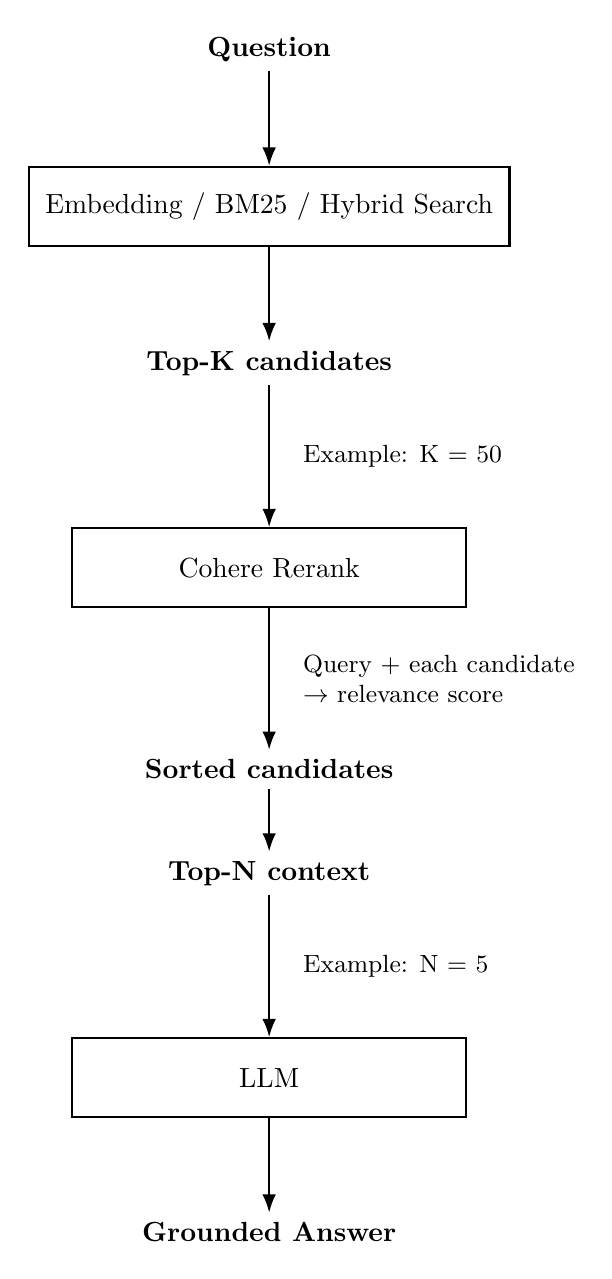
\begin{tikzpicture}[
    % Define styles for the nodes and text
    node distance=1.2cm,
    box/.style={draw, rectangle, thick, align=center, minimum width=5cm, minimum height=1cm, inner sep=6pt},
    textnode/.style={align=center, font=\bfseries},
    arrow/.style={-Latex, thick},
    arrowlabel/.style={align=left, font=\small, right=0.3cm}
]

    % Define the nodes
    \node[textnode] (question) {Question};
    
    \node[box, below=of question] (search) {Embedding / BM25 / Hybrid Search};
    
    \node[textnode, below=of search] (topk) {Top-K candidates};
    
    \node[box, below=1.8cm of topk] (rerank) {Cohere Rerank};
    
    \node[textnode, below=1.8cm of rerank] (sorted) {Sorted candidates};
    
    \node[textnode, below=0.8cm of sorted] (topn) {Top-N context};
    
    \node[box, below=1.8cm of topn] (llm) {LLM};
    
    \node[textnode, below=of llm] (answer) {Grounded Answer};

    % Draw the arrows and attach the side labels
    \draw[arrow] (question) -- (search);
    
    \draw[arrow] (search) -- (topk);
    
    \draw[arrow] (topk) -- node[arrowlabel] {Example: K = 50} (rerank);
    
    \draw[arrow] (rerank) -- node[arrowlabel] {Query + each candidate \\ $\rightarrow$ relevance score} (sorted);
    
    \draw[arrow] (sorted) -- (topn);
    
    \draw[arrow] (topn) -- node[arrowlabel] {Example: N = 5} (llm);
    
    \draw[arrow] (llm) -- (answer);
  \end{tikzpicture}
\end{center}

% \begin{verbatim}
% Question
%    |
%    v
% Embedding / BM25 / Hybrid Search
%    |
%    v
% Top-K candidates
%    |
%    |  Example: K = 50
%    v
% Cohere Rerank
%    |
%    |  Query + each candidate
%    |  -> relevance score
%    v
% Sorted candidates
%    |
%    v
% Top-N context
%    |
%    |  Example: N = 5
%    v
% LLM
%    |
%    v
% Grounded Answer
% \end{verbatim}

The values $K=50$ and $N=5$ are examples, not universal recommendations.

The important design principle is:

\[
K_{\text{retrieval}} > N_{\text{final context}}
\]

The first stage casts a wide net. The reranker then narrows that set.

\section{Why Not Simply Increase Top-$K$?}

Suppose the retriever initially returns:

\[
K=5
\]

and the correct chunk is ranked at position 8.

The correct chunk is never seen by the generator.

Increasing $K$ to 20 may recover the correct chunk:

\[
K=20
\]

but now the LLM may receive many irrelevant chunks.

This creates a trade-off:

\begin{center}
\begin{tabular}{p{0.22\textwidth}p{0.32\textwidth}p{0.32\textwidth}}
\toprule
 & \textbf{Advantage} & \textbf{Risk}\\
\midrule
Small $K$ & Less context, lower token cost & May miss relevant information\\
Large $K$ & Better chance of retrieving relevant information & More irrelevant context and higher token usage\\
Reranking & Recovers candidates first, then improves ordering & Adds computation/latency\\
\bottomrule
\end{tabular}
\end{center}

This is why reranking is especially useful when retrieval quality is important and the final LLM context budget is limited.

\section{Reranking and Context Precision}

Reranking is closely connected to the RAG evaluation metric called \textbf{Context Precision}.

Context Precision evaluates whether relevant chunks are ranked above irrelevant chunks in the retrieved context.

The central question is:

\begin{quote}
\textit{Are the useful chunks near the top of the retrieval results?}
\end{quote}

This is different from simply asking whether a useful chunk exists somewhere in the top-$K$.

For example:

\begin{center}
\begin{tabular}{c|c|c}
\textbf{Rank} & \textbf{Chunk} & \textbf{Relevant?}\\
\midrule
1 & A & Yes\\
2 & B & Yes\\
3 & C & No\\
4 & D & No\\
5 & E & Yes\\
\bottomrule
\end{tabular}
\end{center}

This is generally better than:

\begin{center}
\begin{tabular}{c|c|c}
\textbf{Rank} & \textbf{Chunk} & \textbf{Relevant?}\\
\midrule
1 & C & No\\
2 & D & No\\
3 & E & Yes\\
4 & A & Yes\\
5 & B & Yes\\
\bottomrule
\end{tabular}
\end{center}

Both retrieve the same number of relevant chunks. The second ordering is worse because irrelevant material occupies the highest ranks.

\subsection{Context Precision Formula}

Ragas describes Context Precision in terms of precision at each rank:

\[
\operatorname{Precision@k}
=
\frac{\operatorname{TruePositives@k}}
{\operatorname{TruePositives@k}+\operatorname{FalsePositives@k}}
\]

The Context Precision metric aggregates these rank-sensitive precision values over the retrieved context.

Conceptually:

\[
\boxed{
\text{Context Precision}
\approx
\text{How strongly relevant chunks are concentrated near the top}
}
\]

Higher is better.

\section{Context Recall}

Context Recall asks a different question:

\begin{quote}
\textit{Did the retrieval process find the information needed to answer the question?}
\end{quote}

It is therefore concerned with \textbf{missing information}.

For example, suppose the reference answer requires three pieces of information:

\begin{enumerate}
    \item Policy applies to remote employees.
    \item Manager approval is required.
    \item Core working hours must be maintained.
\end{enumerate}

If the retrieved context supports only two of these three claims, the context has incomplete recall.

For the LLM-based Ragas formulation:

\[
\boxed{
\text{Context Recall}
=
\frac{\text{reference claims supported by retrieved context}}
{\text{total reference claims}}
}
\]

Thus, in the example:

\[
\text{Context Recall}
=
\frac{2}{3}
\approx 0.67
\]

Higher is better.

\subsection{Why Context Recall Needs a Reference}

Recall is fundamentally about what was \textbf{missed}. To know what was missed, we need some representation of what should have been available.

Ragas can use a reference answer as a proxy for the reference context. It breaks the reference into claims and checks whether those claims can be attributed to the retrieved context.

There are also non-LLM and ID-based variants when explicit reference contexts or identifiers are available.

\section{Context Precision vs. Context Recall}

The distinction is critical:

\begin{center}
\begin{tabular}{p{0.25\textwidth}p{0.30\textwidth}p{0.30\textwidth}}
\toprule
 & \textbf{Context Precision} & \textbf{Context Recall}\\
\midrule
Main question & Did we rank useful chunks high? & Did we retrieve the required information?\\
Primary concern & Irrelevant context / bad ordering & Missing relevant information\\
Focus & Precision of retrieved ranking & Completeness of retrieval\\
Reference & Can use reference answer/context & Requires a reference or ground truth representation\\
Higher score & Better & Better\\
Typical remedy & Better ranking, reranking, retrieval tuning & Larger candidate pool, better embeddings, hybrid search, better chunking\\
\bottomrule
\end{tabular}
\end{center}

Thus, 
\\
\textbf{Precision: ``Did I retrieve the right things near the top?''}\\[4pt]
\textbf{Recall: ``Did I retrieve everything important?''}

\section{A Simple Example}

Suppose the correct answer requires three chunks:

\[
R = \{A,B,C\}
\]

The retriever returns:

\[
[A,D,E,B,F,C]
\]

All three relevant chunks were retrieved.

Therefore, context recall is high:

\[
\text{Recall} = \frac{3}{3}=1.0
\]

But the relevant chunks are not all near the top.

If a reranker produces:

\[
[A,B,C,D,E,F]
\]

the set of retrieved information has not changed, but the ordering has improved substantially.

This illustrates an important point:

\begin{quote}
\textbf{Reranking can improve retrieval quality without discovering new documents.}
\end{quote}

The first-stage retriever determines the candidate set. The reranker improves the ordering of that candidate set.

\section{Putting the Metrics and Reranker Together}

A useful conceptual pipeline is:
\\

\begin{center}
    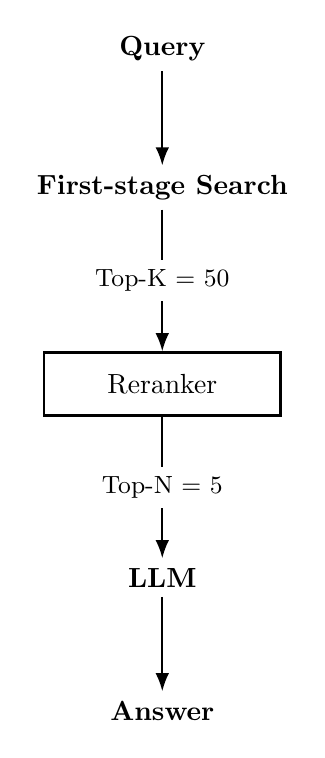
\begin{tikzpicture}[
    % Define styles for the nodes and paths
        node distance=1.2cm,
        box/.style={draw, rectangle, thick, align=center, minimum width=3cm, minimum height=0.8cm},
        textnode/.style={align=center, font=\bfseries},
        arrow/.style={-Latex, thick}
    ]
    
        % Define the nodes
        \node[textnode] (query) {Query};
        
        \node[textnode, below=of query] (search) {First-stage Search};
        
        \node[box, below=1.8cm of search] (reranker) {Reranker};
        
        \node[textnode, below=1.8cm of reranker] (llm) {LLM};
        
        \node[textnode, below=of llm] (answer) {Answer};
    
        % Draw the arrows with inline labels
        \draw[arrow] (query) -- (search);
        
        \draw[arrow] (search) -- node[fill=white, font=\small] {Top-K = 50} (reranker);
        
        \draw[arrow] (reranker) -- node[fill=white, font=\small] {Top-N = 5} (llm);
        
        \draw[arrow] (llm) -- (answer);
    \end{tikzpicture}
\end{center}
% \begin{verbatim}
%                     Query
%                       |
%                       v
%               First-stage Search
%                       |
%                  Top-K = 50
%                       |
%                       v
%                 +-----------+
%                 | Reranker  |
%                 +-----------+
%                       |
%                 Top-N = 5
%                       |
%                       v
%                     LLM
%                       |
%                       v
%                    Answer
% \end{verbatim}

During evaluation:
\\
\begin{center}
  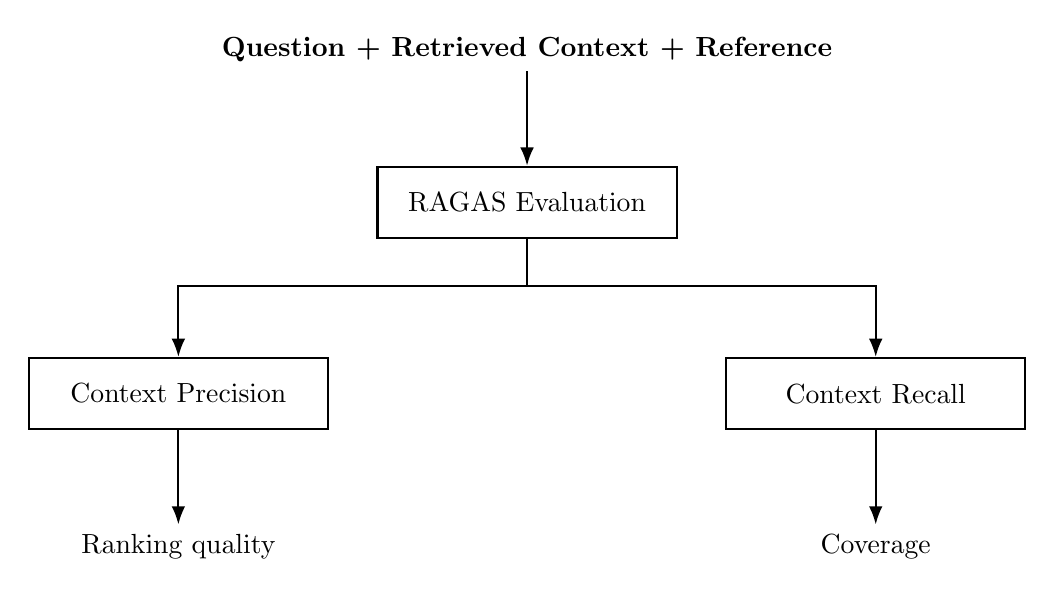
\begin{tikzpicture}[
    % Define common styles
        node distance=1.2cm,
        box/.style={draw, rectangle, thick, align=center, minimum width=3.8cm, minimum height=0.9cm, inner sep=6pt},
        textnode/.style={align=center, font=\bfseries},
        subnode/.style={align=center, font=\normalfont},
        arrow/.style={-Latex, thick}
    ]
    
        % Top input node
        \node[textnode] (input) {Question + Retrieved Context + Reference};
        
        % RAGAS Evaluation box
        \node[box, below=of input] (ragas) {RAGAS Evaluation};
        
        % Split branch nodes
        \node[box, below left=1.5cm and 0.6cm of ragas] (precision) {Context Precision};
        \node[box, below right=1.5cm and 0.6cm of ragas] (recall) {Context Recall};
        
        % Bottom metric description nodes
        \node[subnode, below=of precision] (ranking) {Ranking quality};
        \node[subnode, below=of recall] (coverage) {Coverage};
    
        % Draw main input arrow
        \draw[arrow] (input) -- (ragas);
        
        % Draw the orthogonal branching arrows
        \draw[arrow] (ragas.south) -- ++(0,-0.6) -| (precision.north);
        \draw[arrow] (ragas.south) -- ++(0,-0.6) -| (recall.north);
        
        % Draw bottom arrows
        \draw[arrow] (precision) -- (ranking);
        \draw[arrow] (recall) -- (coverage);

    \end{tikzpicture}    
\end{center}

% \begin{verbatim}
% Question + Retrieved Context + Reference
%                          |
%                          v
%                   RAGAS Evaluation
%                          |
%              +-----------+-----------+
%              |                       |
%              v                       v
%       Context Precision       Context Recall
%              |                       |
%              v                       v
%        Ranking quality          Coverage
% \end{verbatim}

The metrics help diagnose different failure modes.

\section{Typical Failure Patterns}

\subsection{High Recall, Low Precision}

The system retrieved the required information, but buried it under irrelevant material.

Example:

\[
\text{Recall}=0.95,\qquad
\text{Precision}=0.45
\]

Possible remedies:

\begin{itemize}
    \item Add a reranker.
    \item Improve first-stage ranking.
    \item Improve query formulation.
    \item Remove noisy or duplicate chunks.
    \item Improve metadata filtering.
\end{itemize}

\subsection{Low Recall, High Precision}

The chunks that were retrieved are useful, but the system failed to retrieve all the information required.

Example:

\[
\text{Recall}=0.45,\qquad
\text{Precision}=0.90
\]

Possible remedies:

\begin{itemize}
    \item Increase the first-stage retrieval $K$.
    \item Improve embeddings.
    \item Consider hybrid search.
    \item Improve chunking.
    \item Improve query expansion or rewriting.
    \item Review metadata filters that may be excluding useful documents.
\end{itemize}

\subsection{Low Recall, Low Precision}

The retrieval system has a broader problem.

Possible causes include:

\begin{itemize}
    \item Poor chunking.
    \item Poor embeddings.
    \item Incorrect metadata.
    \item Weak query formulation.
    \item Inappropriate vector distance/search configuration.
    \item Poor source-document extraction.
\end{itemize}

Reranking alone will not solve this if the correct information never reaches the reranker.

\section{An Important Limitation of Reranking}

Reranking is not magic.

Suppose the correct chunk is not among the first-stage candidates:

\[
\text{Correct chunk} \notin \text{Top-}K
\]

Then:

\[
\text{Reranker cannot rank it}
\]

because it never received it.

This gives the fundamental relationship:

\[
\boxed{
\text{Reranking improves ordering within the candidate set;
it does not replace candidate generation.}
}
\]

Therefore, a strong RAG architecture must optimize both:

\[
\text{Candidate Recall}
\quad+\quad
\text{Candidate Ranking}
\]

\section{Reranking Is Not the Same as Increasing Top-$K$}

These two techniques solve different problems.

\begin{longtable}{p{0.25\textwidth}p{0.30\textwidth}p{0.30\textwidth}}
\toprule
\textbf{Technique} & \textbf{What it changes} & \textbf{Primary effect}\\
\midrule
Increase Top-$K$ & Expands the candidate set & Potentially improves recall\\
Reranking & Reorders the candidate set & Improves precision/order\\
Improve embeddings & Changes semantic representation & Can improve candidate retrieval\\
Hybrid search & Combines lexical and semantic signals & Can improve recall for exact and semantic matches\\
Better chunking & Changes retrieval units & Can improve both recall and precision\\
\bottomrule
\end{longtable}

In production RAG systems, these techniques are often combined.

\section{Reranking and Token Budget}

A practical reason for reranking is context-budget management.

Suppose:

\[
K=50
\]

retrieved candidates contain approximately 40,000 tokens in total.

It may be impossible or undesirable to send all 50 candidates to the generator.

A reranker can select:

\[
N=5
\]

high-value chunks, producing a much smaller final context.

The conceptual optimization is:

\[
\text{High candidate recall}
\longrightarrow
\text{High relevance}
\longrightarrow
\text{Small final context}
\]

This can reduce:

\begin{itemize}
    \item Input token usage.
    \item Latency.
    \item Context noise.
    \item The chance that the LLM focuses on irrelevant information.
\end{itemize}

Cohere's current Rerank documentation also supports reranking large candidate sets, subject to endpoint and model limits.

\section{Where Reranking Sits in the Bootcamp}

The bootcamp's RAG sequence is deliberately structured around this progression:

\begin{enumerate}
    \item \textbf{Embeddings} --- understand semantic representation.
    \item \textbf{Vector database} --- understand candidate retrieval.
    \item \textbf{Top-$K$} --- understand the recall/context trade-off.
    \item \textbf{RAG pipeline} --- connect retrieval to generation.
    \item \textbf{Context Precision and Context Recall} --- measure retrieval quality.
    \item \textbf{Reranking} --- introduce a second-stage relevance model.
\end{enumerate}

This naturally leads to the broader RAGOps lesson:

\begin{quote}
\textbf{Do not tune a RAG system by changing Top-$K$ blindly. Measure what retrieval is doing.}
\end{quote}

The bootcamp plan explicitly identifies Context Precision and Context Recall as RAG evaluation topics, and the later continuous-evaluation material uses evaluation metrics as a quality gate for AI-system changes.

\section{A Practical Mental Model}

Below is a layman's way to understand the contrast between the two:
\begin{center}
\begin{tabular}{p{0.680\textwidth}p{0.32\textwidth}}
\toprule
\textbf{Question} & \textbf{System component}\\
\midrule
Where might the answer be? & First-stage retriever\\
Which retrieved chunk is most relevant? & Reranker\\
Did we retrieve enough of the required information? & Context Recall\\
Did we rank useful chunks above noisy chunks? & Context Precision\\
How do we turn the context into an answer? & Generative LLM\\
\bottomrule
\end{tabular}
\end{center}

\section{Key Takeaways}

\begin{enumerate}
    \item \textbf{Reranking is a second-stage retrieval technique.}
    \item Cohere provides dedicated \textbf{Rerank models} rather than requiring a general-purpose chat LLM to rank documents.
    \item Cohere Rerank directly considers the \textbf{query and candidate document together} and produces relevance scores.
    \item The first-stage retriever should generally be optimized for \textbf{recall}.
    \item The reranker should improve \textbf{precision and ordering} within the retrieved candidate set.
    \item Increasing Top-$K$ can improve the chance of finding the right information, but it also increases noise.
    \item Reranking cannot recover a document that the first-stage retriever never returned.
    \item \textbf{Context Precision} measures whether relevant retrieved chunks are ranked highly.
    \item \textbf{Context Recall} measures whether the retrieved context contains the information needed to support the reference answer.
    \item Good RAG systems therefore need both \textbf{candidate recall} and \textbf{high-quality ranking}.
\end{enumerate}

\section{One-Sentence Summary}

\begin{quote}
\textbf{Retrieve broadly, rerank precisely, pass only the strongest context to the LLM, and measure retrieval quality using Context Precision and Context Recall.}
\end{quote}

\section{References and Further Reading}

\begin{enumerate}
    \item Cohere, ``Cohere's Rerank Model (Details and Application).''\\
    \url{https://docs.cohere.com/v2/docs/rerank}

    \item Cohere, ``Best Practices for using Rerank.''\\
    \url{https://docs.cohere.com/docs/reranking-best-practices}

    \item Cohere, ``Master Reranking with Cohere Models.''\\
    \url{https://docs.cohere.com/v2/docs/reranking-with-cohere}

    \item Ragas Documentation, ``Context Precision.''\\
    \url{https://docs.ragas.io/en/stable/concepts/metrics/available_metrics/context_precision/}

    \item Ragas Documentation, ``Context Recall.''\\
    \url{https://docs.ragas.io/en/stable/concepts/metrics/available_metrics/context_recall/}
\end{enumerate}

\vfill

\begin{center}
\small
\textcopyright\ 2026 Sujeet Banerjee. All rights reserved.\\
Agentic AI Bootcamp -- Educational material.
\end{center}

\end{document}
